\section{Background}

The introduction framed open-vocabulary and reasoning segmentation as a response to three pressures in dense visual prediction, including fixed label spaces, expensive dense annotation, and the mismatch between predefined class names and natural-language user intent. This section expands that framing before the method taxonomy is introduced. We first compare the major segmentation paradigms by their assumptions and limitations. We then summarize the development axes that organize recent work. We finally define the task family and clarify the boundary between this survey and related lines of review.

\subsection{Segmentation paradigms from closed-set to reasoning}

The development of language-aware segmentation can be broadly divided into four paradigms. The first is closed-set dense prediction. In this setting, the model is trained and evaluated on a fixed vocabulary, and each pixel, instance, or panoptic region is assigned to one predefined category. FCNs~\citep{long2015fully}, Mask R-CNN~\citep{he2017mask}, and panoptic segmentation~\citep{kirillov2019panoptic} made semantic, instance, and panoptic segmentation measurable under fixed datasets, categories, and metrics. The limitation is structural. Once the vocabulary is fixed, the model cannot naturally handle unseen categories, user-defined labels, fine-grained parts, or application-specific concepts without additional annotation or retraining. This limitation motivates methods that treat language as part of the recognition interface.

The second paradigm is open-vocabulary segmentation. Instead of treating the label set as a closed classifier head, open-vocabulary methods use textual category names or natural-language prompts to define recognition targets. Mask-adapted CLIP~\citep{liang2023ovseg}, SAN~\citep{xu2023san}, and ODISE~\citep{xu2023odise} are early examples that move image-text semantics toward dense prediction. Recent work further explores pixel-level alignment, universal segment embeddings, label-free adaptation, and fine-grained semantic alignment~\citep{xshanOpenvocabularySemanticSegmentation2024,xwangUseUniversalSegment2024,shinhOpenvocabularySemanticSegmentation2024,yxchngAligningVisionLanguageModel2026}. This paradigm directly addresses vocabulary openness, but it introduces a tension between semantic breadth and spatial precision. Image-level vision-language representations are strong at recognizing concepts, whereas segmentation requires boundary accuracy, small-object sensitivity, and reliable mask-level discrimination. This tension explains why open vocabularies alone are not sufficient.

The third paradigm is promptable and grounded segmentation. Promptable segmentation separates mask generation from semantic classification. Points, boxes, masks, or language prompts guide a mask generator, and a subsequent grounding or classification component assigns meaning to the mask. SAM~\citep{kirillov2023sam} and SAM2~\citep{ravi2024sam2} make this separation influential by providing class-agnostic mask priors that can be combined with open-vocabulary recognition or language prompting. Recent SAM-based systems extend these priors toward open-vocabulary and universal segmentation~\citep{xhanBoostingSegmentAnything2025,hwangXSAMSegmentAnything2026,sgxiaoOpenworldsamExtendingSam22026}. Grounded segmentation further tightens the connection between language units and spatial regions through region-word alignment, mask-text matching, and grounded multimodal interaction~\citep{xuPixelalignedLanguageModel2024,zhangLlavagroundingGroundedVisual2024,youFerretReferGround2024,rasheedGlammPixelGrounding2024}. This paradigm improves user interaction and spatial grounding, but composed mask priors, language encoders, and downstream classifiers make assumptions and failure modes harder to compare. The next paradigm adds another source of difficulty.

The fourth paradigm is reasoning segmentation. Here the target is not merely a named category or an explicit referring expression. It may need to be inferred from implicit instructions, commonsense, spatial relations, domain rules, or multi-step reasoning. LISA~\citep{lai2024lisa}, PixelLM~\citep{renPixellmPixelReasoning2024}, and GLaMM~\citep{rasheed2024glamm} connect multimodal language understanding with mask prediction through segmentation tokens, pixel decoders, and grounded conversation. Newer work explores agentic reasoning, RL, preference optimization, and hallucination-aware grounding to improve the consistency between textual reasoning and pixel-level evidence~\citep{luoConnectingDotsTrainingFree2026,zhuLensLearningSegment2026,zhuPopenPreferencebasedOptimization2025,zhouReasoningImplicitSelfsupervised2026,guoSeeingBelievingRichContext2026}. This paradigm addresses language flexibility, but it also raises the hardest evaluation question. A response may be linguistically plausible while the produced mask is spatially wrong. The development axes below show how these four paradigms relate.

\subsection{Development of vision-language foundation models for segmentation}

Fig.~\ref{figbackgrounddevelopmentaxes} summarizes the development logic used in this survey. The figure is schematic rather than quantitative. It shows how the field expands along three axes. The semantic space moves from fixed class IDs to text labels, prompts, instructions, and reasoning queries. The spatial unit moves from per-pixel classification toward masks, regions, grounded phrases, and eventually video or 3D entities. The reasoning source moves from task-specific decision rules toward MLLM-based reasoning, agentic decomposition, RL, and verification. These axes provide the reading coordinates for the method taxonomy.

\begin{figure}[t]
    \centering
    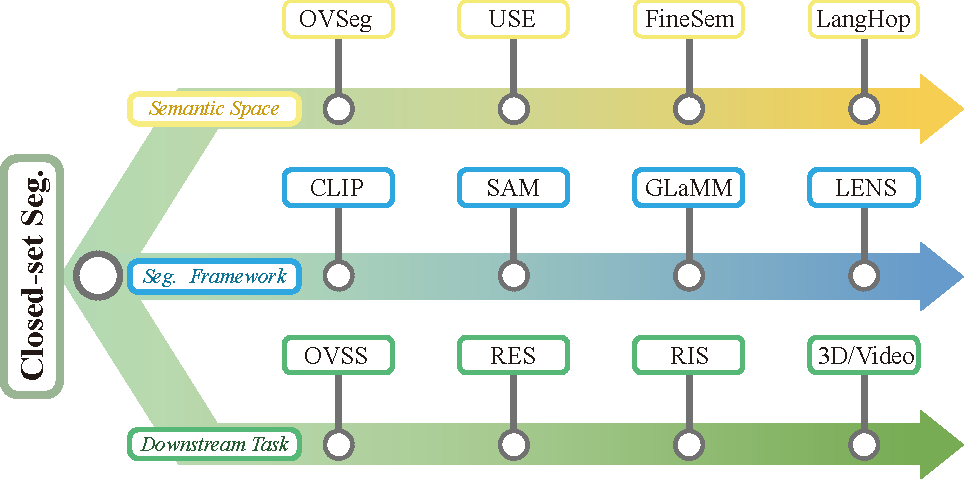
\includegraphics[width=0.98\linewidth]{Fig/background_development_axes.pdf}
    \caption{Illustration of development axes in open-vocabulary and reasoning segmentation. The three arrows summarize how the semantic space, segmentation framework, and downstream task setting evolve from closed-set segmentation toward language-defined vocabularies, unified or composed vision-language systems, and reasoning-intensive scenario grounding.}
    \label{figbackgrounddevelopmentaxes}
\end{figure}

Along the first axis, CLIP~\citep{radford2021learning} style semantic transfer and dense alignment methods adapt image-text representations to pixel or mask prediction. Some methods directly refine visual embeddings for open-vocabulary semantic segmentation. Others use universal segment embeddings, label-free training signals, or fine-grained semantic alignment to improve category transfer~\citep{xshanOpenvocabularySemanticSegmentation2024,xwangUseUniversalSegment2024,shinhOpenvocabularySemanticSegmentation2024,yxchngAligningVisionLanguageModel2026}. These methods establish the basic premise of the field. Text can define the target vocabulary at inference time. Their main challenge is that the alignment learned for image-level recognition does not automatically produce reliable dense localization. This challenge leads to mask-centric frameworks.

Along the second axis, segmentation foundation models and mask-centric pipelines make spatial priors more explicit. SAM~\citep{kirillov2023sam} and SAM2~\citep{ravi2024sam2} based methods use promptable masks as a reusable spatial substrate, then combine them with open-vocabulary classifiers, language prompts, or grounded interaction modules~\citep{xhanBoostingSegmentAnything2025,hwangXSAMSegmentAnything2026,sgxiaoOpenworldsamExtendingSam22026}. This route is powerful because it decouples where an object may be from what the object is. However, decoupling also creates a dependency on proposal quality, prompt design, mask filtering, and the calibration between mask confidence and semantic confidence.

Along the third axis, grounded and reasoning systems connect mask prediction with language generation or structured decision processes. Region-word and mask-text methods make the grounding unit more explicit, while MLLM-based systems add conversational and instruction-following capabilities~\citep{xuPixelalignedLanguageModel2024,zhangLlavagroundingGroundedVisual2024,youFerretReferGround2024,rasheed2024glamm}. Reasoning-oriented work then pushes the task from explicit reference resolution toward implicit target discovery, reward-guided grounding, and hallucination detection~\citep{lai2024lisa,renPixellmPixelReasoning2024,zhuLensLearningSegment2026,guoSeeingBelievingRichContext2026}. These developments explain why benchmark design must evaluate not only mask overlap, but also whether the visual evidence actually supports the language rationale.

\subsection{Task family and terminology}

Several task names in this area are closely related but not interchangeable. Open-vocabulary semantic segmentation asks a model to assign each pixel to categories that may include unseen or user-provided labels. Open-vocabulary instance and panoptic segmentation add object identity or stuff/thing structure, so the model must both discover regions and assign them to an open label space. These tasks primarily test semantic openness under dense prediction.

Promptable segmentation refers to mask generation conditioned on user prompts such as points, boxes, masks, or text. Its output can be class-agnostic or later assigned to semantic labels. Referring expression segmentation instead assumes that the target is specified by a phrase or sentence, and the output is the mask corresponding to the referred object or region. Grounded segmentation generalizes this idea by linking words, phrases, generated responses, or conversational turns to spatial regions. These tasks primarily test the binding between language units and masks.

Reasoning segmentation goes one step further. The target may be implicit and must be inferred before it can be segmented. The query can involve commonsense, spatial relations, false premises, task constraints, medical or remote-sensing rules, affordance, or multi-turn interaction. This makes reasoning segmentation a joint test of language understanding, visual grounding, and mask generation rather than a pure segmentation benchmark. Recent extensions to video, 3D scenes, remote sensing, medicine, affordance, and embodied grounding stress-test whether the same assumptions hold beyond static 2D natural images~\citep{xuVideosegr1ReasoningVideo2026,chen3DDRESDetailed3D2026,libExploringEfficientOpenvocabulary2026,yanMedreasonerReinforcementLearning2026,wangAffordancer1ReinforcementLearning2026}. These task definitions prepare the section-level taxonomy used by the rest of the survey.

Fig.~\ref{figbackgroundtaxonomy} gives the section-level taxonomy used in the remainder of this survey. The taxonomy follows the rule that categories should be organized by objective, framework, setup, task, and grounding mechanism rather than by paper chronology. Sections~5 to~8 cover the major method families, Section~9 compares their assumptions and benchmark limitations, and Section~10 turns those limitations into future directions.

\begin{figure*}[t]
    \centering
    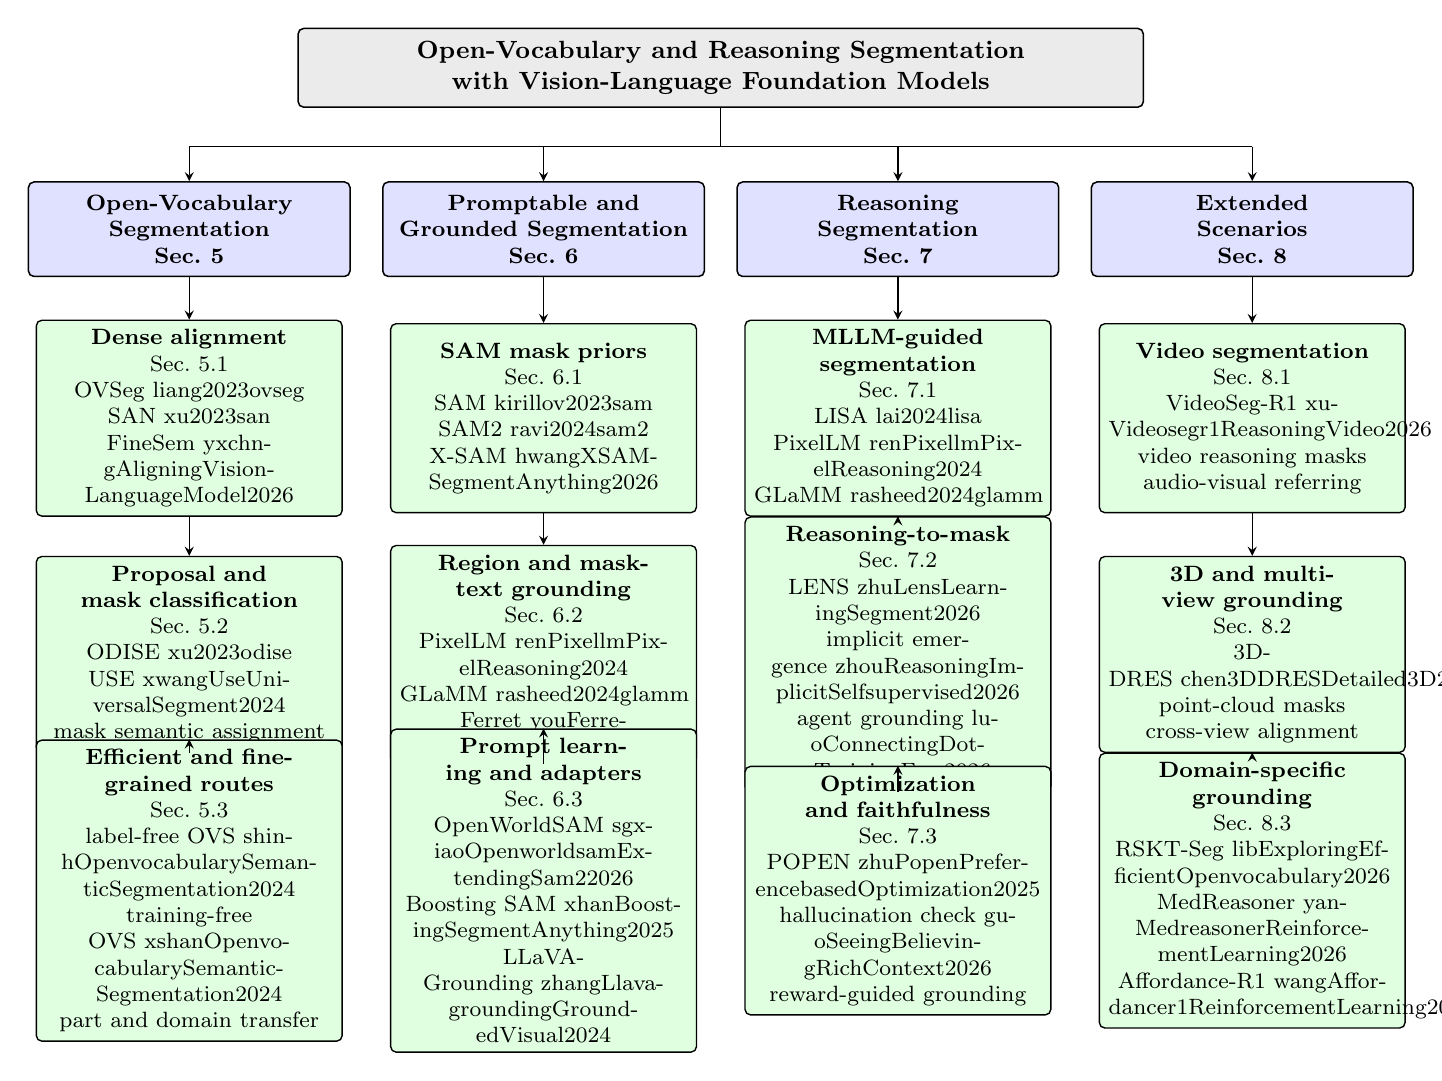
\begin{tikzpicture}[
        x=1cm,
        y=1cm,
        rootbox/.style={draw, rounded corners=2pt, fill=black!8, line width=0.55pt, align=center, text width=10.5cm, minimum height=1cm, font=\small\bfseries},
        % 调整了 headbox 的 minimum height
        headbox/.style={draw, rounded corners=2pt, fill=blue!12, line width=0.55pt, align=center, text width=3.85cm, minimum height=1.2cm, font=\footnotesize\bfseries},
        % 调整了 itembox 的 minimum height 为 2.4cm，确保所有方框一样高
        itembox/.style={draw, rounded corners=2pt, fill=green!12, line width=0.50pt, align=center, text width=3.65cm, minimum height=2.4cm, font=\footnotesize},
        link/.style={line width=0.45pt},
        arrowlink/.style={link, ->, >=stealth}
    ]
        \node[rootbox] (root) at (9.0,8.8) {Open-Vocabulary and Reasoning Segmentation\\with Vision-Language Foundation Models};

        \coordinate (bus) at (9.0,7.8);
        \coordinate (busleft) at (2.25,7.8);
        \coordinate (busright) at (15.75,7.8);
        \draw[link] (root.south) -- (bus);
        \draw[link] (busleft) -- (busright);

        \node[headbox] (h1) at (2.25,6.75) {Open-Vocabulary\\Segmentation\\Sec.~5};
        \node[headbox] (h2) at (6.75,6.75) {Promptable and\\Grounded Segmentation\\Sec.~6};
        \node[headbox] (h3) at (11.25,6.75) {Reasoning\\Segmentation\\Sec.~7};
        \node[headbox] (h4) at (15.75,6.75) {Extended\\Scenarios\\Sec.~8};

        \draw[arrowlink] (2.25,7.8) -- (h1.north);
        \draw[arrowlink] (6.75,7.8) -- (h2.north);
        \draw[arrowlink] (11.25,7.8) -- (h3.north);
        \draw[arrowlink] (15.75,7.8) -- (h4.north);

        % --- 调整下方节点的 y 坐标，大幅拉开纵向间距 ---
        
        % 第一行 y = 4.00 (原为 5.05)
        \node[itembox] (ov1) at (2.25,4.35) {\textbf{Dense alignment}\\Sec.~5.1\\OVSeg~\citep{liang2023ovseg}\\SAN~\citep{xu2023san}\\FineSem~\citep{yxchngAligningVisionLanguageModel2026}};
        \node[itembox] (pg1) at (6.75,4.35) {\textbf{SAM mask priors}\\Sec.~6.1\\SAM~\citep{kirillov2023sam}\\SAM2~\citep{ravi2024sam2}\\X-SAM~\citep{hwangXSAMSegmentAnything2026}};
        \node[itembox] (rs1) at (11.25,4.35) {\textbf{MLLM-guided segmentation}\\Sec.~7.1\\LISA~\citep{lai2024lisa}\\PixelLM~\citep{renPixellmPixelReasoning2024}\\GLaMM~\citep{rasheed2024glamm}};
        \node[itembox] (ex1) at (15.75,4.35) {\textbf{Video segmentation}\\Sec.~8.1\\VideoSeg-R1~\citep{xuVideosegr1ReasoningVideo2026}\\video reasoning masks\\audio-visual referring};

        % 第二行 y = 1.00 (原为 3.35)
        \node[itembox] (ov2) at (2.25,1.35) {\textbf{Proposal and mask classification}\\Sec.~5.2\\ODISE~\citep{xu2023odise}\\USE~\citep{xwangUseUniversalSegment2024}\\mask semantic assignment};
        \node[itembox] (pg2) at (6.75,1.35) {\textbf{Region and mask-text grounding}\\Sec.~6.2\\PixelLM~\citep{renPixellmPixelReasoning2024}\\GLaMM~\citep{rasheed2024glamm}\\Ferret~\citep{youFerretReferGround2024}};
        \node[itembox] (rs2) at (11.25,1.35) {\textbf{Reasoning-to-mask}\\Sec.~7.2\\LENS~\citep{zhuLensLearningSegment2026}\\implicit emergence~\citep{zhouReasoningImplicitSelfsupervised2026}\\agent grounding~\citep{luoConnectingDotsTrainingFree2026}};
        \node[itembox] (ex2) at (15.75,1.35) {\textbf{3D and multiview grounding}\\Sec.~8.2\\3D-DRES~\citep{chen3DDRESDetailed3D2026}\\point-cloud masks\\cross-view alignment};

        % 第三行 y = -2.00 (原为 1.65)
        \node[itembox] (ov3) at (2.25,-1.65) {\textbf{Efficient and fine-grained routes}\\Sec.~5.3\\label-free OVS~\citep{shinhOpenvocabularySemanticSegmentation2024}\\training-free OVS~\citep{xshanOpenvocabularySemanticSegmentation2024}\\part and domain transfer};
        \node[itembox] (pg3) at (6.75,-1.65) {\textbf{Prompt learning and adapters}\\Sec.~6.3\\OpenWorldSAM~\citep{sgxiaoOpenworldsamExtendingSam22026}\\Boosting SAM~\citep{xhanBoostingSegmentAnything2025}\\LLaVA-Grounding~\citep{zhangLlavagroundingGroundedVisual2024}};
        \node[itembox] (rs3) at (11.25,-1.65) {\textbf{Optimization and faithfulness}\\Sec.~7.3\\POPEN~\citep{zhuPopenPreferencebasedOptimization2025}\\hallucination check~\citep{guoSeeingBelievingRichContext2026}\\reward-guided grounding};
        \node[itembox] (ex3) at (15.75,-1.65) {\textbf{Domain-specific grounding}\\Sec.~8.3\\RSKT-Seg~\citep{libExploringEfficientOpenvocabulary2026}\\MedReasoner~\citep{yanMedreasonerReinforcementLearning2026}\\Affordance-R1~\citep{wangAffordancer1ReinforcementLearning2026}};

        \draw[arrowlink] (h1.south) -- (ov1.north);
        \draw[arrowlink] (ov1.south) -- (ov2.north);
        \draw[arrowlink] (ov2.south) -- (ov3.north);
        \draw[arrowlink] (h2.south) -- (pg1.north);
        \draw[arrowlink] (pg1.south) -- (pg2.north);
        \draw[arrowlink] (pg2.south) -- (pg3.north);
        \draw[arrowlink] (h3.south) -- (rs1.north);
        \draw[arrowlink] (rs1.south) -- (rs2.north);
        \draw[arrowlink] (rs2.south) -- (rs3.north);
        \draw[arrowlink] (h4.south) -- (ex1.north);
        \draw[arrowlink] (ex1.south) -- (ex2.north);
        \draw[arrowlink] (ex2.south) -- (ex3.north);
    \end{tikzpicture}
    \caption{Taxonomy and section mapping for this survey. The main method sections are organized into open-vocabulary segmentation, promptable and grounded segmentation, reasoning segmentation, and extended scenarios. The bottom row links this taxonomy to the comparison axes and future directions used later in the manuscript.}
    \label{figbackgroundtaxonomy}
\end{figure*}

\subsection{Relation to existing surveys}

This survey is positioned as a task-centered review of recent open vocabulary and reasoning segmentation rather than a general review of VLMs, segmentation foundation models, or MLLMs. Broader VLM reviews usually emphasize pre-training objectives, image-level recognition, retrieval, or general multimodal reasoning. Segmentation foundation model discussions often focus on promptable mask generation and adaptation. Open vocabulary segmentation discussions usually center on category transfer and dense semantic alignment. These perspectives are useful, but they do not fully explain how open label spaces, promptable masks, grounded language interaction, and reasoning-to-mask generation interact in the same evaluation landscape.

Our boundary is therefore narrower in topic but broader in comparison. We focus on methods that produce, align, or evaluate pixel-level or region-level masks under open-vocabulary, promptable, grounded, or reasoning settings. We do not claim that this is the first survey of any individual subfield. Instead, the goal is to provide a shared map for comparing task assumptions, supervision forms, foundation backbones, prompt formats, output types, datasets, and evaluation protocols across the rapidly converging literature. This boundary also determines the later organization. Foundations and datasets are introduced before methods, method families are compared after their mechanisms are reviewed, and future directions are derived from the benchmark and grounding gaps identified along the way.
